\chapter{NCBI accession numbers}
\section{Bacterial single cells}
Raw sequencing data on \textit{E. coli} and \textit{S. aureus} are accessible at the NCBI Sequence Read Archive (SRA) under BioProject accession number PRJNA279815 with BioSample accession numbers SAMN03451478-SAMN03451501. FijiCOMP metagenomic reads can be found under BioProject accession number PRJNA217052 with the accession numbers: SRX345831, SRX344363, SRX344765, SRX343094, SRX344442, SRX346405, SRX343839, SRX343780, SRX345901, SRX344600, SRX343866, SRX343411, SRX344189, SRX344380, SRX346966, SRX345329, SRX343800, and SRX344616. FijiCOMP \textit{virtual microfluidics} 117 single cells are accessible with the BioSample accession numbers SAMN04461233-SAMN04461349.

\section{Human single cells}
Raw sequencing data on RPE-1 bulk genomic DNA and single cells using \textit{virtual microfluidics} are accessible under BioProject accession number PRJNA408301 with BioSample accession numbers SAMN07682898 and SAMN07682891. 

\begin{table}
\caption{SRA accession numbers for human single-cell chimera analysis}
\label{tab:SRAaccession}
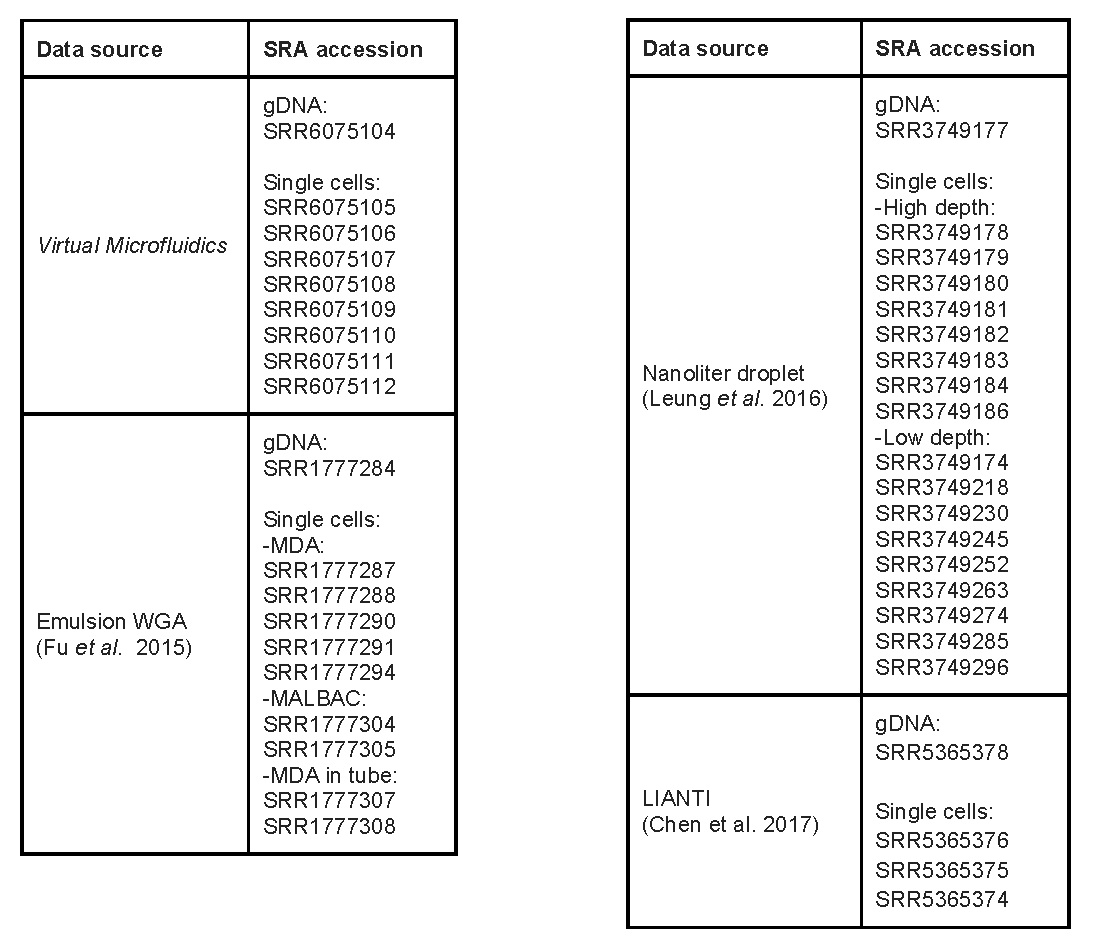
\includegraphics[width=0.8\linewidth]{./figures/SRAaccession}
\end{table}

% \begin{table}
% \centering 
% \caption{QPCR characterization of hydrogel punches}
% \label{tab:QpcrHydrogel}
% \begin{adjustbox}{max width=0.7\textwidth}
% \begin{tabular}{c||c} 

% \hline 
% Total hydrogel punches & 80 \\ 
% \hline
% \textit{E. coli} positive punches & 7  \\
% \hline
% \textit{S. aureus} positive punches & 36 \\
% \hline
% Double positive & 7 \\
% \hline
% Double negative & 30 \\
% \hline
% \end{tabular}
% \end{adjustbox}
% \end{table}

% \begin{table}
% \caption{PCR primer sequences}
% \label{tab:ESprimerList}
% \begin{center}
% 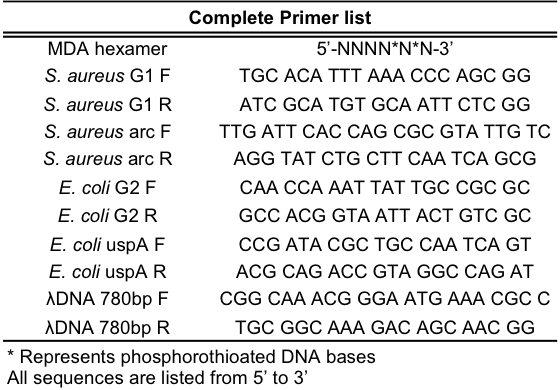
\includegraphics[width=0.5\linewidth]{./figures/ESprimerList}
% \end{center}
% \end{table}

% \begin{table}
% \caption{Mapping statistics, \textit{E. coli} and \textit{S. aureus}}
% \label{tab:MapStatES}
% 
\includegraphics[width=\linewidth]{./figures/MapStatES}
% \end{table}

% \begin{table}
% \caption{Sequence read classification \say{other reads}, \textit{E. coli} and \textit{S. aureus}}
% \label{tab:OtherReadsES}
% 
\includegraphics[width=\linewidth]{./figures/OtherReadsClassificationES}
% \end{table}

% \begin{table}
% \caption{Downsampling on mapped reads from single-cell MDA samples}
% \label{tab:DownsamplingESD}
% 
\includegraphics[width=\linewidth]{./figures/DownsamplingESdeBourcy}
% \end{table}

% \begin{table}
% \caption{Metagenomic shotgun profiling weighted with single-cell samples}
% \label{tab:MetagenomicFiji}
% 
\includegraphics[width=\linewidth]{./figures/MetagenomicShotgunProfilingFiji}
% \end{table}

% \begin{table}
% \caption{Data source for chimera analysis}
% \label{tab:chimeraDataSource}
% \includegraphics[width=\linewidth]{./figures/Chimera_DataSource}
% \end{table}

% \begin{table}
% \caption{Single-cell technology comparisons for chimera analysis}
% \label{tab:chimeraTechTable}
% 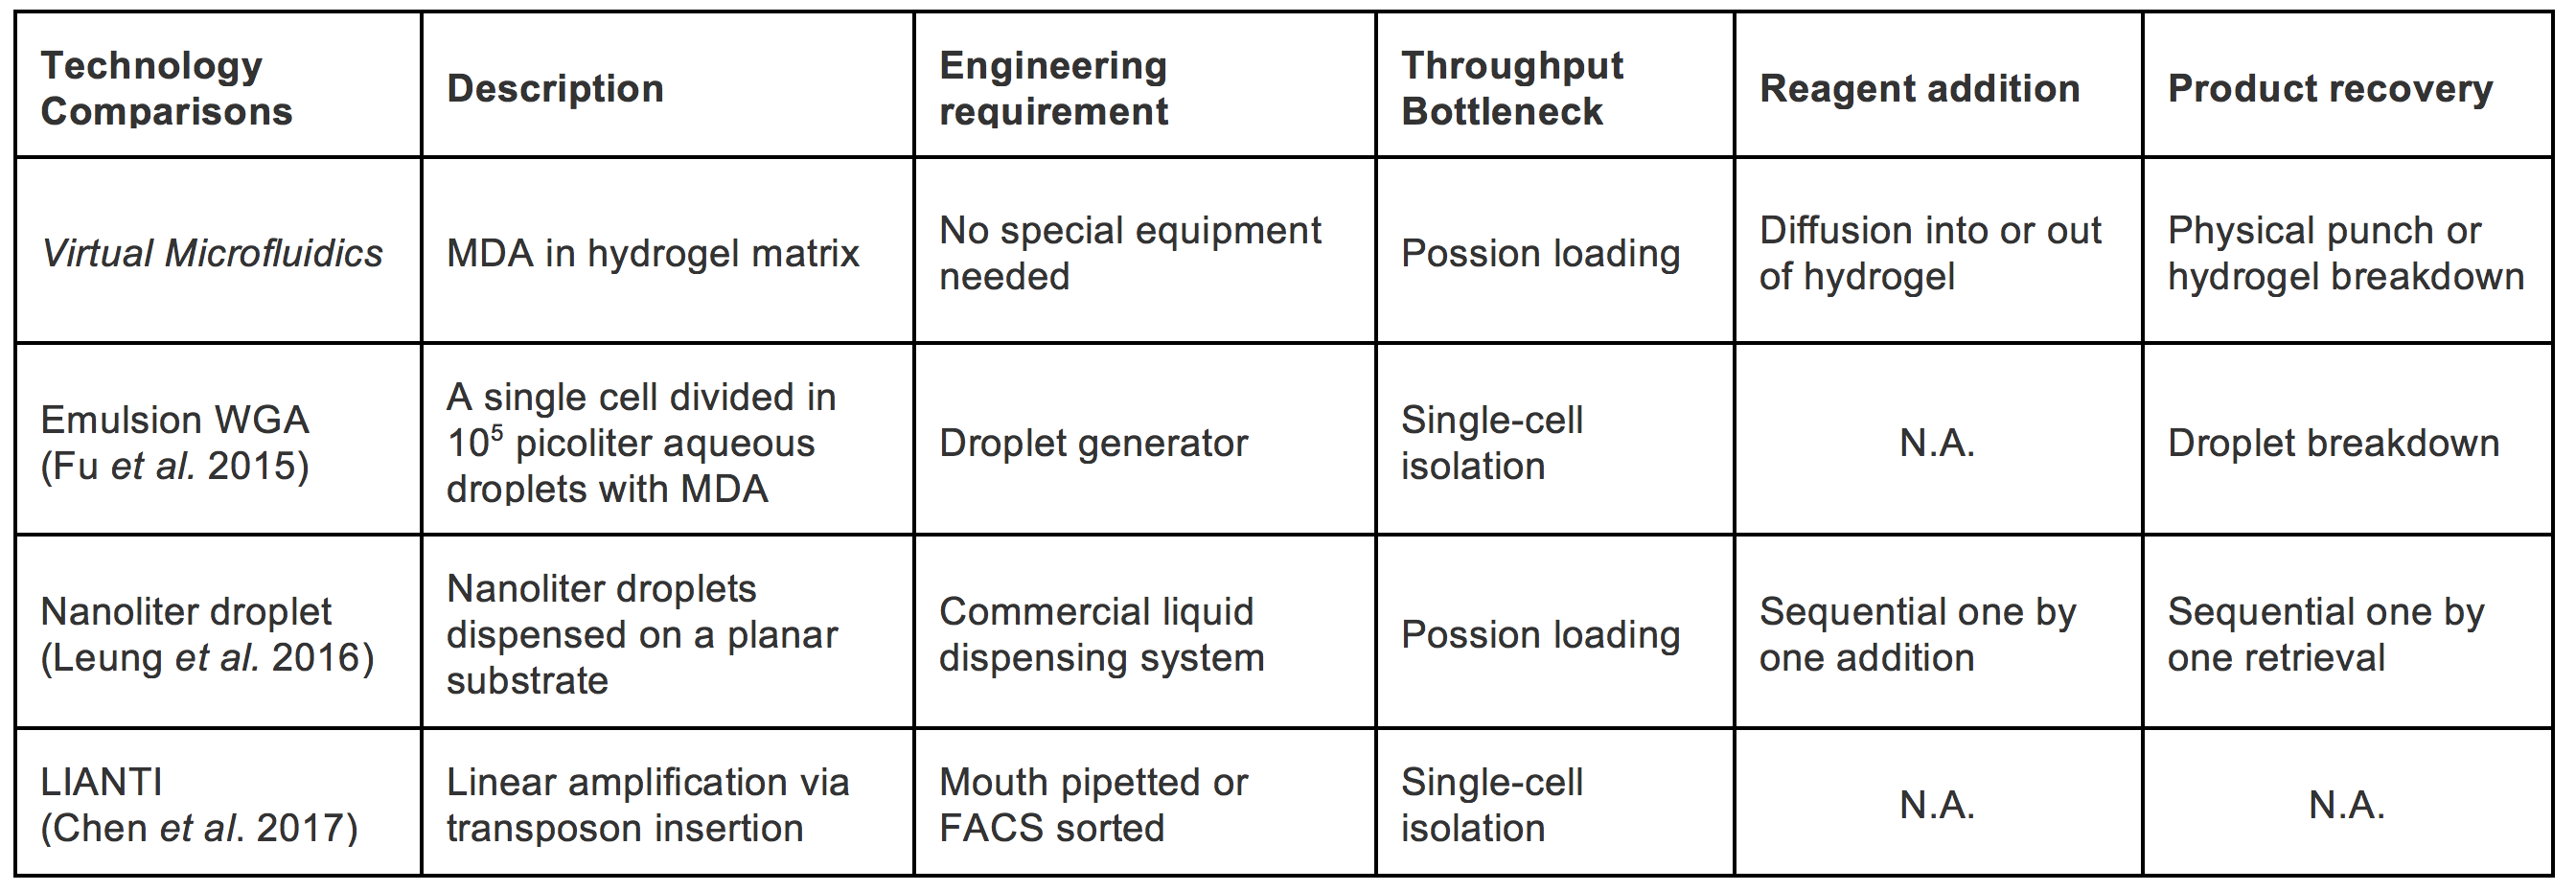
\includegraphics[width=\linewidth]{./figures/Chimera_TechTable}
% \end{table}

\clearpage